\chapter{Helmholtz -- 2D -- Acoustic Waves -- Air in a Cavity}

\modinfo{Directory}{AcousticWaves}
\modinfo{Solvers}{\Idx{Helmholtz}}
\modinfo{Tools}{\Idx{ElmerGUI}}
\modinfo{Dimensions}{2D,Steady State}
\modinfo{Author}{Peter R{\aa}back}


\subsection*{Introduction}

Elmer provides two alternative ways of conducting acoustic analyses in the frequency domain. Firstly, one may simply use the Helmholtz equation which is based on the assumption of lossless flow, i.e.\ the effects of viscosity and heat conduction are assumed to be negligible. More refined analyses where these effects are taken into account may be carried out by using the specific solver for the set of time-harmonic dissipative acoustic equations. The aim of this tutorial is to demonstrate the usage of the solver for the basic Helmholtz equation, which is frequently taken as the starting point in acoustic analyses. 

\subsection*{Case definition}

\begin{wrapfigure}{r}{0.45\textwidth}
\centering
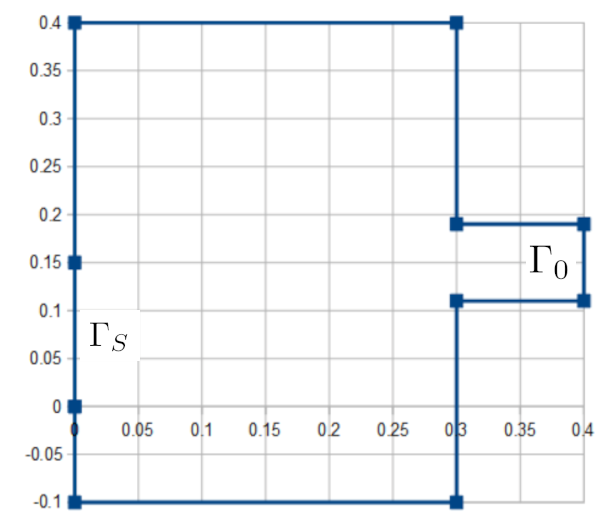
\includegraphics[width=0.45\textwidth]{geometry}
\caption{Geometry}\label{fg:geometry}
\end{wrapfigure}

In this problem the fluctuations of the pressure in an air-filled cavity shown in Figure~\ref{fg:geometry} are considered. The cavity is connected with the surrounding air by an open narrow pipe. The pressure fluctuations are generated by a vibrating membrane on the boundary $\Gamma_S$ with the frequency of the motion being $f=100$ Hz.  The remaining parts of the boundary are assumed to be rigid walls. In addition, the effects of gravity are assumed to be negligible.

Suitable boundary conditions in terms of the pressure must be given. On the rigid walls the pressure flux is prescribed to vanish which corresponds to the assumption that there is no velocity in the direction normal to the boundary. At the open end $\Gamma_0$ the impedance boundary condition suitable for forward travelling plane waves is given by setting $Z=-c$ with $c$ being the sound speed. We assume that $c=343$ (m/s). Finally, the wave source is given by defining a non-vanishing pressure flux on the corresponding part of the boundary. We take simply $\nabla P \cdot \vec n = 1$ where $P$ is the (complex) amplitude of the pressure and $\vec n$ is the outward unit normal to the boundary. 

\subsection*{ElmerGUI Equation Menu}

We will be using the \Idx{Helmholtz Solver}, which is one of the default, pre-loaded GUI definitions, so it does not need to be manually activated.  For reference, the  \texttt{\Idx{helmholtz.xml}} definition file is, by default, located in Linux in:

\texttt{\$ELMER\_HOME/share/ElmerGUI/edf}\\

and in Windows, located in:

\texttt{C:/Program Files/Elmer 9.0-Release/share/ElmerGUI/edf}\\

\subsection*{Solution procedure}

\begin{wrapfigure}{r}{0.4\textwidth}
\centering
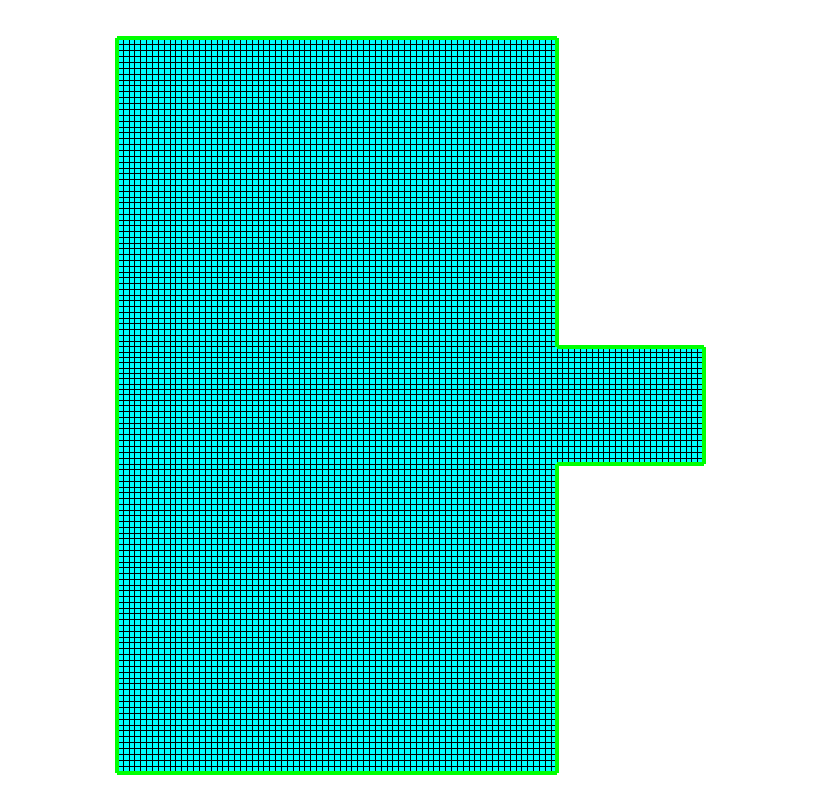
\includegraphics[width=0.4\textwidth]{mesh}
\caption{Mesh.}\label{fg:mesh}
\end{wrapfigure}

The mesh is given in ElmerGrid format in file \texttt{domain.grd}, load this file.

\ttbegin
File 
  Open -> domain
\ttend

You should obtain your mesh and may check \texttt{Model Summary...} that it consists of 10050 surface elements.  Your mesh should look like as shown in figure \ref{fg:mesh}

After we have the mesh we start to go through the Model menu from the top to bottom.  In the Setup we choose things related to the whole simulation such as file names, time stepping, constants etc.  

The simulation is carried out in 2-dimensional Cartesian coordinates.

\ttbegin
Model
  Setup 
    Simulation Type = Steady state
    Steady state max. iter = 1
  Apply
\ttend

In the equation section we choose the relevant equations and parameters related to their solution. 

In this case we'll have one equation (named ``Helmholtz'').

When defining Equations and Materials it is possible to assign to the bodies immediately, or to use mouse selection to assign them later. In this case we have just one body and therefore its easier to assign the Equation and Material to it directly.\\

For the linear system solvers we are happy to use the defaults. One may however, try out different preconditioners (ILU1,\ldots) or direct Umfpack solver, for example.

\ttbegin
Model
  Equation
   Name = Helmholtz
    Apply to Bodies = 1
    Helmholtz Equation
      Active = on
      Angular Frequency = 628.3
      Convection Velocity 1 = 0.0
      Convection Velocity 2 = 0.0
    Add 
    OK
\ttend        
The Material section includes all the material parameters. They are divided into generic parameters which are direct properties of the material without making any assumptions on the physical model, such as the mass. Other properties assume a physical law, such as conductivities and viscosity. 

\ttbegin
Model
  Material
    Apply to Bodies = 1 
    General 
      Density = 1.224
    Helmholtz
      Damping coefficient = 0.0
      Sound speed = 343
    Add
    OK
\ttend

A Body Force represents the right-hand-side of a equation. It is generally not a required field for a body, and is not needed for this example.

Initial conditions should be given to transient cases, and probably are not needed for steady state solutions, and is not needed for this example.

Only one boundary condition may be applied to each boundary and therefore all the different physical BCs for a boundary should be grouped together. 

The conditions may be assigned to boundaries in the Boundary condition menu, or by clicking on each boundary with the mouse. Here we use the first approach since there are only three boundaries.

\ttbegin
Model
  BoundaryCondition
    Name = Constraint1
    Boundary 1 is checked
    Helmholtz Equation
      Flux conditions
        Real part of the flux = 1
        Imag part of the flux = 0
    Add
    New

    Name = Constraint2
    Boundary 2 is checked
    Helmholtz Equation
      Flux conditions
        Real part of the flux = 0
        Imag part of the flux = 0
    Add
    New

    Name = Constraint3
    Boundary 3 is checked
    Helmholtz Equation
      Flux conditions
        Real part of the impedance = -343
        Imag part of the impedance = 0
    Add
   OK 
\ttend   

For the execution ElmerSolver needs the mesh files and the command file.  We have now basically defined all the information for ElmerGUI to write the command file. After writing it we may also visually inspect the command file.
\ttbegin
Sif 
  Generate
  Edit -> look how your command file came out  
\ttend

Before we can execute the solver we should save the files in a directory.  The ElmerGUI project includes all the files needed to restart the case.

\ttbegin
File 
  Save Project
\ttend

After we have successfully saved the files we may start the solver.

\ttbegin
Run
  Start solver
\ttend

A convergence view automatically pops up showing relative changes of each iteration.

When there are some results to view we may start the postprocessor also.

\ttbegin
Run
  Start ParaView
\ttend

\subsection*{Results}

The difference of the maximum of (0.32) and the minimum (0.21) value of the pressure is found to be $\Delta p \approx 0.11$

You may inspect the results with Paraview or with ElmerVTK.\\

In Figure \ref{fg:press-mag} the obtained pressure wave magnitude is presented.  In Figure \ref{fg:press-xy} the obtained pressure wave in the x-direction and y-direction is presented. 

\begin{figure}[H]
\centering
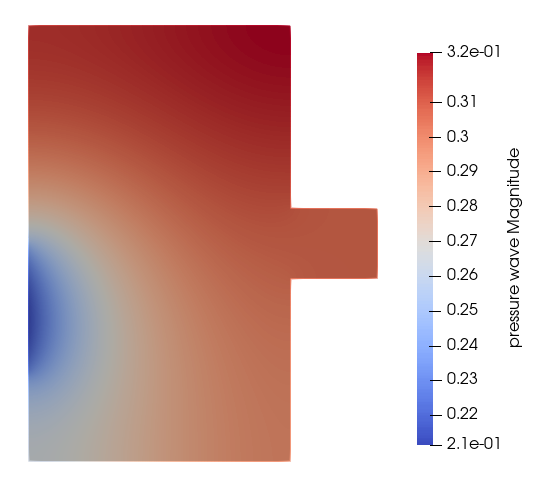
\includegraphics[width=0.65\textwidth]{press-mag}
\caption{Pressure wave magnitude}\label{fg:press-mag}
\end{figure} 

\begin{figure}[H]
\centering
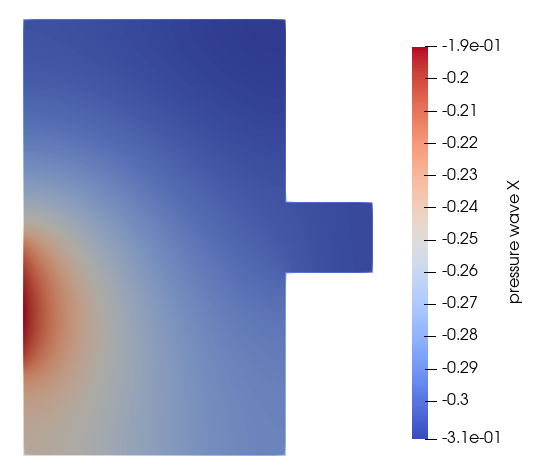
\includegraphics[width=0.48\textwidth]{press-x}
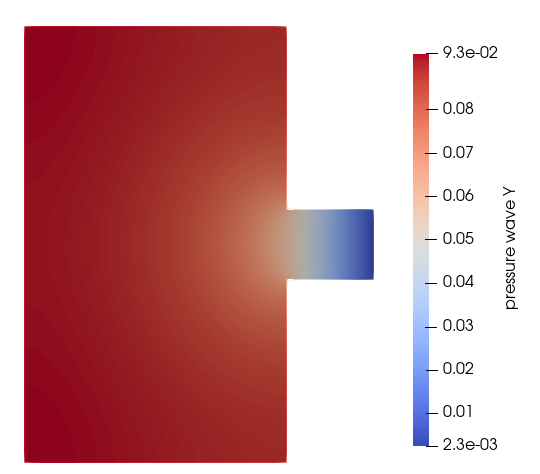
\includegraphics[width=0.48\textwidth]{press-y}
\caption{Pressure wave, x-direction, and y-direction}\label{fg:press-xy}
\end{figure} 

\subsection*{Extra task:}

If you have time you may try to solve the case with different parameters.

\hfill
